%%%%%%%%%%%%%%%%%%%%%%%%%%%%%%%%%%%%%%%%%%%%%%%%%%%%%%%%%%%%%%%%%%%%%%%%%%%%%%%%
% Medium Length Graduate Curriculum Vitae
% LaTeX Template
% Version 1.2 (3/28/15)
%
% This template has been downloaded from:
% http://www.LaTeXTemplates.com
%
% Original author:
% Rensselaer Polytechnic Institute 
% (http://www.rpi.edu/dept/arc/training/latex/resumes/)
%
% Modified by:
% Daniel L Marks <xleafr@gmail.com> 3/28/2015
%
% Important note:
% This template requires the res.cls file to be in the same directory as the
% .tex file. The res.cls file provides the resume style used for structuring the
% document.
%
%%%%%%%%%%%%%%%%%%%%%%%%%%%%%%%%%%%%%%%%%%%%%%%%%%%%%%%%%%%%%%%%%%%%%%%%%%%%%%%%

%-------------------------------------------------------------------------------
%	PACKAGES AND OTHER DOCUMENT CONFIGURATIONS
%-------------------------------------------------------------------------------

%%%%%%%%%%%%%%%%%%%%%%%%%%%%%%%%%%%%%%%%%%%%%%%%%%%%%%%%%%%%%%%%%%%%%%%%%%%%%%%%
% You can have multiple style options the legal options ones are:
%
%   centered:	the name and address are centered at the top of the page 
%				(default)
%
%   line:		the name is the left with a horizontal line then the address to
%				the right
%
%   overlapped:	the section titles overlap the body text (default)
%
%   margin:		the section titles are to the left of the body text
%		
%   11pt:		use 11 point fonts instead of 10 point fonts
%
%   12pt:		use 12 point fonts instead of 10 point fonts
%
%%%%%%%%%%%%%%%%%%%%%%%%%%%%%%%%%%%%%%%%%%%%%%%%%%%%%%%%%%%%%%%%%%%%%%%%%%%%%%%%

\documentclass[overlapped]{res} 

% Default font is the helvetica postscript font
\usepackage{helvet}
\usepackage{textcomp}
\usepackage{url}
\usepackage{hyperref}
\usepackage{xcolor}
\usepackage[margin=0.7in]{geometry} % Set 1in margin or adjust as needed
\usepackage{graphicx}
\usepackage{fontawesome5}
\usepackage{tabularx}



\newcommand{\pink}[1]{\textcolor{pink!40!red}{#1}} % Adjust the percentage as needed


% Increase text height
\textheight=720pt

\begin{document}

%-------------------------------------------------------------------------------
%	NAME AND ADDRESS SECTION
%-------------------------------------------------------------------------------
% \name{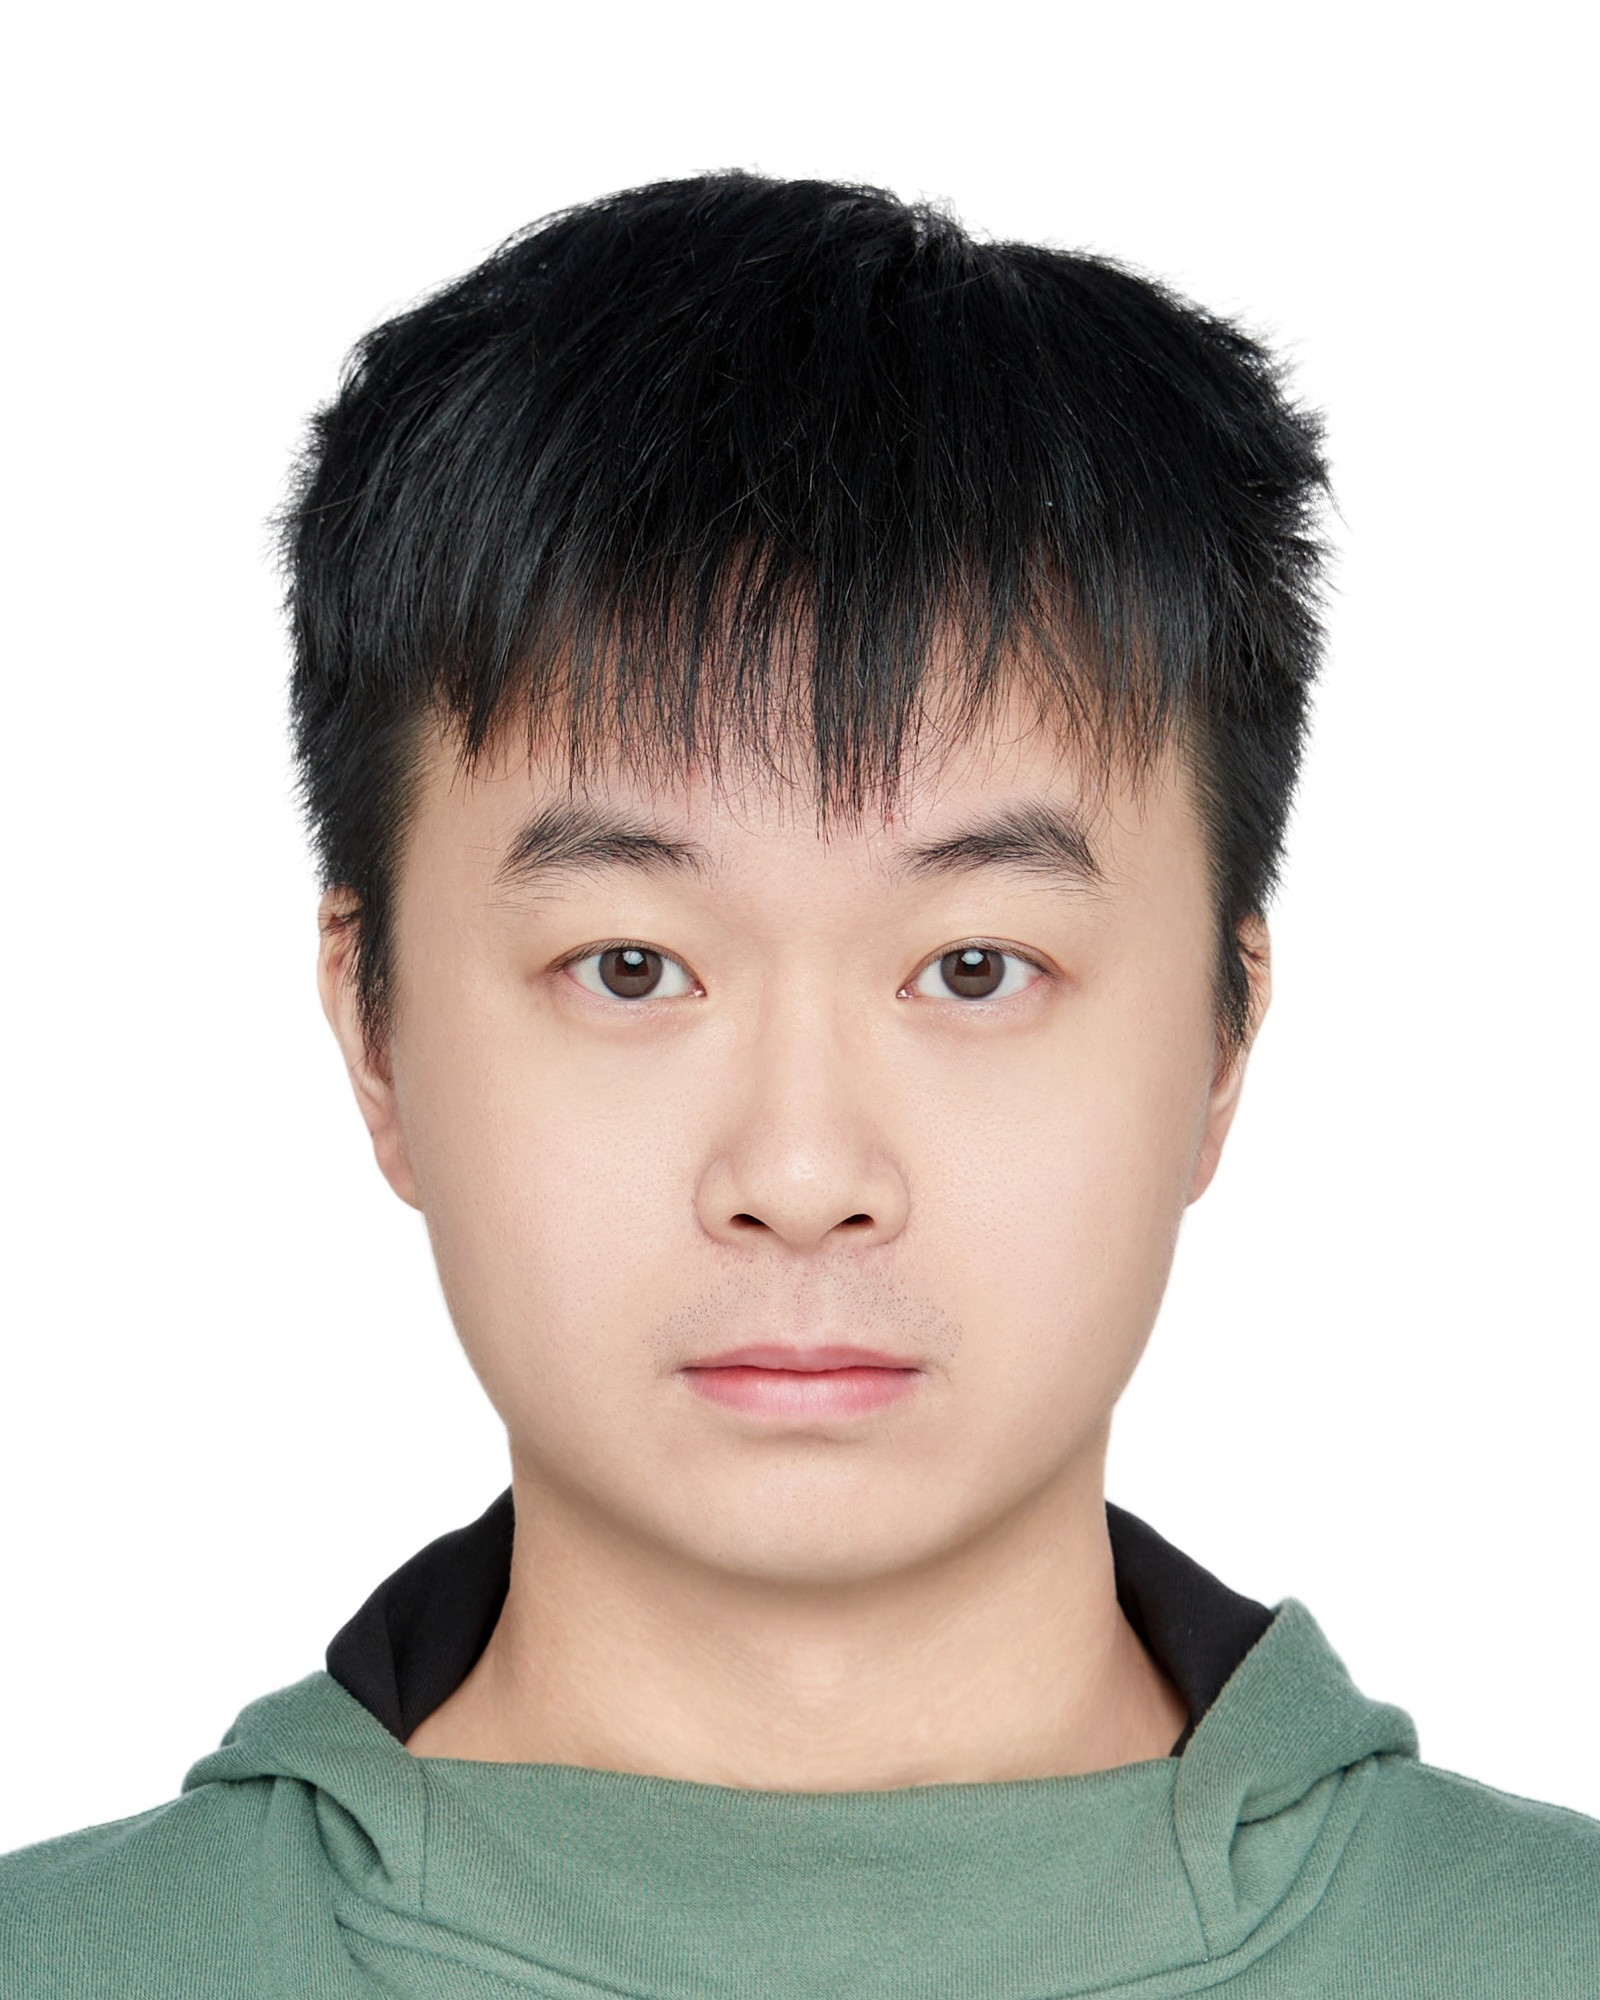
\includegraphics[width=1in, height=1in, keepaspectratio]{mugshot.jpg}\\Patrick Li-Yu Lo}
\name{Patrick Li-Yu Lo}

% Note that addresses can be used for other contact information:
% -phone numbers
% -email addresses
% -linked-in profile

\address{134B, North Building\\Research Dr, Durham NC}
\address{\hfill
\href{https://www.linkedin.com/in/patrick-li-yu-lo-700600185/}{\faLinkedin}
\href{mailto:patrick.lo@duke.edu}{\faEnvelope}
\href{https://scholar.google.com/citations?hl=en\&user=RwZlE9AAAAAJ\&view\_op=list\_works\&sortby=pubdate}{\faGraduationCap}
\href{https://github.com/pattylo}{\faGithub} 
\\ \pink{\texttt{\url{https://pattylo.github.io/}}}
} 

% Uncomment to add a third address
%\address{Address 3 line 1\\Address 3 line 2\\Address 3 line 3}
%-------------------------------------------------------------------------------

\begin{resume}

\begin{format}
  \title{l}\dates{r}\\
  % \employer{l}\location{r}\\
  \body\\
\end{format}

%-------------------------------------------------------------------------------
%	EDUCATION SECTION
%-------------------------------------------------------------------------------
\section{BACKGROUND}
\textbf{Duke University} \hfill Aug \textquotesingle{}25 - Present\\
PhD Student in Robotics (Mechanical Engineering) \hfill GPA: 3.88/4.0
\\\\
\textbf{The Hong Kong Polytechnic University} \hfill Sep \textquotesingle{}22 - Mar \textquotesingle{}25\\
MPhil in Robotics \& Control (Presidential Fellow) \hfill GPA: 4.0/4.3
% Department of Aeronautical and Aviation Engineering
% \textbf{Thesis}: On Improving the  of Controllers and Estimators for Mobile Robots in Challenging Operational Conditions
\\ \\ 
\textbf{Hong Kong Center for Construction Robotics (HKCRC)} \hfill Jul \textquotesingle{}21 - Jul \textquotesingle{}22\\
Research Assistant
\\\\
\textbf{The Hong Kong Polytechnic University} \hfill Sep \textquotesingle{}17 - Jun \textquotesingle{}21\\
BEng (1st Hons) in Aeronautical and Aviation Engineering (APEC Entry Scholarship) \hfill GPA: 3.75/4.3
\\\\
\textbf{The University of Queensland, Australia} \hfill Feb \textquotesingle{}20 - Jul \textquotesingle{}20\\
Exchange Student
\par\noindent\hrule width \linewidth % Horizontal line limited to the width of the page

% \section{RESEARCH EXPERIENCE }
% \textbf{Adaptive Control for Underactuated Robots leveraging Koopman Operators and Reinforcement Learning for Dynamic Robustness} \hfill \textit{\textbf{Sep 2024 - Present}}\\
% \textit{Research Assistant} 
% % Dr. Carlos Mastalli (Heriot-Watt)
% \begin{itemize}
%   \setlength{\itemsep}{-0.4pt} % Adjust the spacing here
%   \item Designed an adaptive framework to address data insufficiency in Koopman operator-based controllers.
%   \item Developed a policy network for optimizing controller parameters.
%   \item Demonstrating the framework's performance through simulations and physical experiments.
% \end{itemize}
% %%%%%%%%%%%%%%%%%%%%%%%%%%%%%%%%%%%%%%%%%%%%%%%%%%%%%%
% \textbf{Improving and Optimizing Adaptive Controllers via Disturbances Observers and Reinforcement Learning} \hfill \textit{\textbf{Aug 2023 - Aug 2024}}\\
% \textit{MPhil Student} 
% \begin{itemize}
%   \setlength{\itemsep}{-0.4pt} % Adjust the spacing here
%   \item Proposed an adaptive framework for MPC, LQR, and EKF on mobile robots using disturbance observation.
%   \item Improved, analyzed, and implemented General ESO (GESO) and Error-State ESO (ESESO) for lump disturbance estimation.
%   \item Developed reinforcement learning (RL) for parameter optimization.
%   \item Demonstrated performance on UUV MPC control, heterogeneous UAV-UGV relative state estimation, and multi-UAV sliding-mode control (SMC).
% \end{itemize}
% %%%%%%%%%%%%%%%%%%%%%%%%%%%%%%%%%%%%%%%%%%%%%%%%%%%%%%
% \textbf{Non-Robocentric Dynamic Landing for Quadrotor UAVs} \hfill \textit{\textbf{Sep 2022 - Jul 2023}}\\
% \textit{MPhil Student} 
% \begin{itemize}
%   \setlength{\itemsep}{-0.4pt} % Adjust the spacing here
%   \item Proposed a non-inertial autonomous dynamic landing framework without using airborne exteroceptive sensors.
%   \item Developed an IEKF-based state estimator on SE(3).
%   \item Designed kinematic and dynamic constrained trajectories using differential flatness and minimized jerk.
%   \item Demonstrated system applicability via physical experiments using a self-designed UAV-UGV hardware system.
% \end{itemize}
% \par\noindent\hrule width \linewidth % Horizontal line limited to the width of the page
% % \setlength{\baselineskip}{0.4\baselineskip}

% \section{WORK EXPERIENCE}
% \textbf{PolyU AAE Department} \hfill \textit{\textbf{Feb 2025 - Now}}\\
% \textit{Research Administrative Assistant}
% \begin{itemize}
%   \setlength{\itemsep}{-0.4pt}
%   \item Designed and developed a prototype unmanned underwater vehicle (UUV), including integration of sensors and embedded control software for autonomous navigation.
%   \item Contributed to the editing and proofreading of an academic textbook, ensuring technical accuracy, consistency in terminology, and clarity in the presentation of complex engineering concepts.
% \end{itemize}
% \textbf{Hong Kong Center for Construction Robotics (HKCRC)} \hfill \textit{\textbf{Jul 2021 - Jul 2022}}\\
% \textit{Research Assistant}
% \begin{itemize}
%   \setlength{\itemsep}{-0.4pt}
%   \item Developed a learning-based model via adversarial training and data augmentation for a CV-based construction logistics monitoring system.
%   \item Developed PID controllers and EKF estimators for an automation system aiding prefabrication component installation, currently pending patent.
% \end{itemize}
% \par\noindent\hrule width \linewidth % Horizontal line limited to the width of the page
%-------------------------------------------------------------------------------

%	PROJECTS SECTION
%-------------------------------------------------------------------------------
\section{PUBLICATIONS \& PATENTS 
% (\pink{\texttt{\href{https://pattylo.github.io/pdfs/research_ppt.pdf}{SLIDES}}})
}
\textbf{First-Author Publications}
% $^{\dagger}$ Co-first authors.
\begin{itemize}
  \item \underline{\textbf{L.-Y. Lo}}$^{\dagger}$, Y. Liu$^{\dagger}$, C. Shu, T. Harris, J. Ryan, and B. Chen, ``Fly, drive, reconfigure: A modular reconfigurable aerial-ground platform for field operations,'' \textit{arXiv preprint arXiv:2609.28887}, 2026. \textit{Links}: \pink{\texttt{\href{https://pattylo.github.io/pdfs/harp.pdf}{pdf}}}, \pink{\texttt{\href{https://github.com/generalroboticslab/HARP}{code}}}.
  \item N. Weaver$^{\dagger}$, B. Xia$^{\dagger}$, \underline{\textbf{L.-Y. Lo}}$^{\dagger}$, Y. Huang, and B. Chen, ``Omnidirectional amphibious locomotion via internal mass actuation,'' \textit{arXiv preprint arXiv:2609.27358}, 2026. \textit{Links}: \pink{\texttt{\href{https://pattylo.github.io/pdfs/ballbot.pdf}{pdf}}}, \pink{\texttt{\href{https://github.com/generalroboticslab/MARBLE}{code}}}.
  \item \underline{\textbf{L.-Y. Lo}}, B. Li, C.-Y. Wen, and C.-W. Chang, ``Experimental non-robocentric dynamic landing of quadrotor UAVs with on-ground sensor suite,'' \textit{IEEE Transactions on Instrumentation and Measurement (TIM)}, vol. 73, 2024. \textit{Links}: \pink{\texttt{\href{https://pattylo.github.io/pdfs/tim.pdf}{pdf}}}, \pink{\texttt{\href{https://github.com/HKPolyU-UAV/ALAN}{code}}}.
  \item \underline{\textbf{L.-Y. Lo}}, Y. Hu, B. Li, C.-Y. Wen, and Y. Yang, ``An adaptive model predictive control for unmanned underwater vehicles subject to external disturbances and measurement noise,'' in \textit{2024 14th Asian Control Conference (ASCC)}. IEEE, 2024, pp. 01–07. \textit{Links}: \pink{\texttt{\href{https://pattylo.github.io/pdfs/uuv.pdf}{pdf}}}, \pink{\texttt{\href{https://github.com/HKPolyU-UAV/bluerov2/tree/eskf_obs2}{code}}}.
  \item \underline{\textbf{L.-Y. Lo}}, B. Li, C.-Y. Wen, and C.-W. Chang, ``Landing a quadrotor on a ground vehicle without exteroceptive airborne sensors: A non-robocentric framework and implementation,'' in \textit{2023 IEEE 26th International Conference on Intelligent Transportation Systems (ITSC)}. IEEE, 2023, pp. 6080–6087. \textit{Links}: \pink{\texttt{\href{https://pattylo.github.io/pdfs/itsc.pdf}{pdf}}}.
  \item \underline{\textbf{L.-Y. Lo}}, C. H. Yiu, Y. Tang, A.-S. Yang, B. Li, and C.-Y. Wen, ``Dynamic object tracking on autonomous UAV system for surveillance applications,'' \textit{Sensors}, vol. 21, no. 23, p. 7888, 2021. Editor's Choice Article. \textit{Links}: \pink{\texttt{\href{https://pattylo.github.io/pdfs/auto.pdf}{pdf}}}, \pink{\texttt{\href{https://github.com/HKPolyU-UAV/auto}{code}}}.
\end{itemize}
\textbf{Other Publications \& Patents}
\begin{itemize}
  \item Y. Liu, R. Prakash, \underline{\textbf{L.-Y. Lo}}, N. Roede, and B. Chen, ``Embodied passive aeroacoustic perception enables relative sensing and pursuit between aerial robots,'' \textit{arXiv preprint arXiv:2608.00401}, 2026. \textit{Links}: \pink{\texttt{\href{https://pattylo.github.io/pdfs/sonicfly.pdf}{pdf}}}, \pink{\texttt{\href{https://github.com/generalroboticslab/SonicFly}{code}}}.
  \item Y. Yang, K. Liu, \underline{\textbf{L.-Y. Lo}}, T. Huang, Y. Fu, and C.-Y. Wen, “Fixed-time adaptive consensus control for multi-quadrotor subject to external disturbances via deep reinforcement learning,” \textit{Aerospace Science and Technology (AST)}, p. 111133, 2025. \textit{Links}: \pink{\texttt{\href{https://pattylo.github.io/pdfs/swarm_rl.pdf}{pdf}}}.
  \item W. Yang, K. Liu, Z. Tan, \underline{\textbf{L.-Y. Lo}}, Y. Wang, K.-H. Wong, and C.-Y. Wen, “Hierarchical 3D scene graph based semantic-metric SLAM for plant inspection and fruit counting in intelligent hydroponics system,” \textit{IEEE Internet of Things Journal}, 2025. \textit{Links}: \pink{\texttt{\href{https://pattylo.github.io/pdfs/scene_graph.pdf}{pdf}}}.
  
  \item C.-W. Chang, L.K. Chung, W.-C. Hung, and \underline{\textbf{L.-Y. Lo}}, ``An integrated auxiliary system for construction precast components installation,'' Patent Pending, Application No.: 202310478194.5, \textit{CN Patent}, [Filing Date: 2023-08-29].
  
\end{itemize}

\par\noindent\hrule width \linewidth % Horizontal line limited to the width of the page
\section{AWARDS \& SCHOLARSHIP}
\begin{itemize}
  \item First Runner-up of UAV Challenge, \textquotesingle{}23, \textquotesingle{}24, \& \textquotesingle{}25 IEEE International Conference on Unmanned Aircraft Systems (ICUAS). \textit{Links}: \pink{
    \texttt{\href{https://www.polyu.edu.hk/publications/pulse-polyu/issue/202308/achievements/aae-team-wins-first-runner-up-prize-at-icuas-23-uav-competition}{web \textquotesingle{}23}}},
    \pink{
    \texttt{\href{https://www.polyu.edu.hk/aae/news-and-events/news/2024/jun-20_icuas-2024-first-runner-up/}{web \textquotesingle{}24}}},
    \pink{
    \texttt{\href{https://www.polyu.edu.hk/aae/news-and-events/news/2025/20250702_icuas2025/?sc_lang=en}{web \textquotesingle{}25}}}.
  \item PolyU Presidential Postgraduate Fellowship Scheme (\textquotesingle{}22 - \textquotesingle{}24).
  \item Dean’s List of PolyU Faculty of Engineering: \textquotesingle{}17/18, \textquotesingle{}18/19 \& \textquotesingle{}20/21.
  \item PolyU Undergraduate APEC Entry Scholarship (\textquotesingle{}17 - \textquotesingle{}21).
  \item Wong Tit-shing Student Exchange Scholarship \textquotesingle{}19/20.
  \item Dr. Y.K. Ching Memorial Scholarship \textquotesingle{}19.
\end{itemize}
\par\noindent\hrule width \linewidth % Horizontal line limited to the width of the page
%-------------------------------------------------------------------------------
\section{CORE SKILLS \& EXPERIENCES}
\textbf{Languages \& Tools}: C++, Python, ROS 1/2, Matlab, Docker, Arduino, PyTorch, \& OpenCV.\\
\textbf{Expertise}: Nonlinear and Convex Optimization, Dynamics \& Control, Data-Driven Methods, Opt-Based SLAM. \\
\textbf{Robotic Platforms}: PX4/ArduPilot, AgileX Scout-Mini, BlueROV2, CrazyFly, UniTree Go1. \\
\textbf{Links:} \pink{{\texttt{\href{https://pattylo.github.io/\#project}{Project Pages}}}}, \pink{{\texttt{\href{https://github.com/pattylo/learning_jungle}{Learning Notes}}}}.
\par\noindent\hrule width \linewidth % Horizontal line limited to the width of the page
%-------------------------------------------------------------------------------
\section{OTHERS}
\begin{itemize}
  \item \textbf{Languages}: English (C1), Mandarin (Native), Cantonese (Proficient), Taiwanese (Proficient).
  \item \textbf{Reviewing}: CoRL \textquotesingle{}26, IEEE ITSC \textquotesingle{}23; IEEE TIM, TMECH, TVT, Sensors Journal; Nonlinear Dynamics.
\end{itemize}
\par\noindent\hrule width \linewidth
\section{LEADERSHIP \& SERVICE}
\begin{itemize}
  \item \textbf{Leadership}\\
  President, Duke Taiwanese Student Association \hfill \textquotesingle{}26--\textquotesingle{}27\\
  Student Ambassador, HKPolyU \hfill \textquotesingle{}19--\textquotesingle{}21
  \item \textbf{Teaching Assistant}\\
  ME555 Robot Manipulation, Duke University \hfill Sep \textquotesingle{}26\\
  ENG2002 Computer Programming, HKPolyU \hfill Sep \textquotesingle{}23\\
  AAE1BN01 Introduction to Aviation Industry, HKPolyU \hfill Jun \textquotesingle{}23
  \item \textbf{Volunteer Teaching Assistant}\\
  HeartFire Education Service, China \hfill Dec \textquotesingle{}19\\
  African Evangelistic Enterprise, Rwanda \hfill Jun \textquotesingle{}19\\
  Royal University of Phnom Penh, Cambodia \hfill May--Jun \textquotesingle{}18
\end{itemize}
\par\noindent\hrule width \linewidth % Horizontal line limited to the width of the page
\section{REFERENCES}
\vspace{5pt} % Adjust the value for the desired amount of space
\begin{tabularx}{\textwidth}{l l l l}
  Prof. Chih-Yung Wen & Dr. Boyang Li & Dr. Li-Ta Hsu & Dr. Ching-Wei Chang \\
  (+852) 3400 2522 & (+61) 02 4055 0828 & (+852) 3400 8061 & (+852) 6996 1656 \\
  \texttt{cywen@polyu.edu.hk} & \texttt{boyang.li@newcastle.edu.au} & \texttt{lt.hsu@polyu.edu.hk} & \texttt{ccw@ust.hk}
\end{tabularx}






% \textbf{Relative State Estimation for Non-Inertial Control Systems}  
% \hfill \textit{Sep '22 - Aug '24} \\
% We study the relative state estimation problem for the feedback loop of non-inertial control systems (e.g., ground-centralized UAV-UGV heterogeneous teams) based on visual measurements, control input signals, and observed disturbance. 

% \begin{itemize}
%   \item \textbf{Main modules:} Investigated the unknown input problem in Kalman filters; designed adaptive extended state observer to extract the real input; fused the lump disturbance and control input into the prediction model of IEKF; performed stability analysis in the sense of Lyapunov for the observer.
%   \item \textbf{Tools:} C++/Python in ROS, Gazebo, PX4, Docker.
%   % \item \textbf{Achievements:} Paper accepted at \textit{2024 IEEE Asian Control Conference}.
% \end{itemize}

% \textbf{Observer-based MPC for Unmanned Underwater Vehicle}  
% \hfill \textit{Aug '23 - Mar  '24} \\
% We designed a novel error-state extended state observer subject to physical sensor models for adaptive nonlinear UUV MPC. 

% \begin{itemize}
%   \item \textbf{Main modules:} Investigated the IMU model and ESKF; applied Fossen's UUV equation to design the prediction model; integrated the lump disturbance into the prediction model; performed stability analysis in the sense of Lyapunov for both observer and controller.
%   \item \textbf{Tools:} C++/Python in ROS, Gazebo, Acados/Casadi, BlueROV2 SITL, Docker.
%   \item \textbf{Achievements:} Paper accepted at \textit{2024 IEEE Asian Control Conference}.
% \end{itemize}

% \textbf{Towards Non-Robocentric Dynamic Landing for Quadrotor UAVs} 
% \hfill \textit{Jul '22 - Aug  '23} \\
% We proposed a novel sensing configuration for the UAV dynamic landing problem where no airborne exteroceptive sensors were used.

% \begin{itemize}
%   \item \textbf{Main modules:} Carried out stereo camera image processing; proposed IEKF-based state estimator on SE(3); designed kinematic and dynamic constrained trajectory with differential flatness \& minimized jerk; coded PID outer-loop flight controller; conducted heterogeneous UAV-UGV hardware system design and physical experiments in VICON.
%   \item \textbf{Tools:} C++/Python in ROS, Gazebo, OSQP, PX4, Docker.
%   \item \textbf{Achievements:} Paper published in \textit{2023 IEEE International Conference on Intelligent Transportation System}; extended version accepted to \textit{IEEE Transactions on Instrumentation and Measurement}; knowledge transferred (partial) to \textit{HKSAR Environmental Protection Department}.
% \end{itemize}

% \textbf{CV-based Construction Logistics Monitoring System} 
% \\
% Prototyped an enhanced Automatic License Plate Recognition (ALPR) system for trucks on construction sites which was a collaboration project with the industry.

% \begin{itemize}
%   \item \textbf{Main modules:} Conducted literature review on adversarial training; performed data augmentation; conducted image pre-processing; co-designed auxiliary hardware setup for better image captures.
%   \item \textbf{Tools:} PyTorch, Arduino.
%   \item \textbf{Achievements:} Knowledge transferred to \textit{Hong Kong Sun Hung Kai Properties}.
% \end{itemize}

% \textbf{Vision-based Navigation of Quadrotor UAV} 
% \hfill \textit{Aug '20 - May  '21} \\
% We worked on a fully autonomous UAV with SLAM, dynamic object tracking, path planning, trajectory generation, and controller modules. The team specifically focused on SLAM and dynamic object tracking.

% \begin{itemize}
%   \item \textbf{Main modules:} Conducted CNN training for object detection; carried out stereo camera image processing; proposed EKF-based state estimator for object tracking; proposed visual-dynamic sensor fusion with TCN/LSTM models to solve the unknown input problem.
%   \item \textbf{Tools:} C++/Python in ROS, Gazebo, Darknet, OpenCV DNN, PyTorch, GTSAM, PX4.
%   \item \textbf{Achievements:} 2 papers were published in \textit{Sensors} and \textit{Aerospace} as an undergraduate RA; Github repo received $\sim$100 stars.
% \end{itemize}
%-------------------------------------------------------------------------------

%-------------------------------------------------------------------------------
%	EXPERIENCE SECTION
%-------------------------------------------------------------------------------
% Modify the format of each position


% \employer{PTP Turbo Blankets}
% \location{Austin, Texas}
% \dates{May 2014-Present}
% \title{\textbf{Content Marketing}}
% \begin{position}
% I produce our social media content, including some of our graphics. I develope our content strategies and impliment them upon approval. I maintain our company's online presence and showcase our industry expertise by leveraging our presence in the automotive racing and performance community.
% \end{position}
%-------------------------------------------------------------------------------
% \employer{The Hong Kong Polytechnic University}
% \location{Hong Kong}
% \dates{Jun '19 - Dec '23}
% \title{\textbf{Teaching Assistant}}
% \begin{position}
% Course: ENG2002 Computer Programming, Sep-Dec '23; AAE1BN01 Introduction to Aviation Industry, Jun-Aug '23; COMP3S02 Socially Responsible Global Leadership in a Digital World (Rwanda), Jun '19.
% \end{position}

% \employer{IEEE}
% \location{Hong Kong}
% \dates{Sep '22 - Present}
% \title{\textbf{Reviewer}}
% \begin{position}
% Journal/Conference: IEEE Transactions on Mechatronics; IEEE Sensor Journal; 2023 IEEE International Conference on Intelligent Transportation System.
% \end{position}

% \dates{May '18 - Jun '21}
% \title{\textbf{Volunteering}}
% \begin{position}
% Events: Student ambassador of PolyU ('19-'21); Volunteer at HeartFire Education Service (Dec '19), African Evangelistic Enterprise (Jun '19), Royal University of Phnom Penh (May - Jun '18).
% \end{position}

% \dates{}
% % \title{\textbf{Others}}
% \title{}
% \begin{position}
% Languages: English (IELTS 7.5), Mandarin (Native), Cantonese (Proficient), Taiwanese (Proficient).\\
% Hobbies: Guitar; Baseball; Skateboarding.
% \end{position}
% \section{SERVICE \& OTHERS}

% \employer{The Hong Kong Polytechnic University}
% \location{Hong Kong}
% \dates{Jun '19 - Dec '23}
% \title{\textbf{Teaching Assistant}}
% \begin{position}
% Course: ENG2002 Computer Programming, Sep-Dec '23; AAE1BN01 Introduction to Aviation Industry, Jun-Aug '23; COMP3S02 Socially Responsible Global Leadership in a Digital World (Rwanda), Jun '19.
% \end{position}

% \employer{IEEE}
% \location{Hong Kong}
% \dates{Sep '22 - Present}
% \title{\textbf{Reviewer}}
% \begin{position}
% Journal/Conference: IEEE Transactions on Mechatronics; IEEE Sensor Journal; 2023 IEEE International Conference on Intelligent Transportation System.
% \end{position}

% \dates{May '18 - Jun '21}
% \title{\textbf{Volunteering}}
% \begin{position}
% Events: Student ambassador of PolyU ('19-'21); Volunteer at HeartFire Education Service (Dec '19), African Evangelistic Enterprise (Jun '19), Royal University of Phnom Penh (May - Jun '18).
% \end{position}

% \dates{}
% \title{\textbf{Others}}
% \begin{position}
% Languages: English (IELTS 7.5), Mandarin (Native), Cantonese (Proficient), Taiwanese (Proficient).\\
% Hobbies: Guitar; Baseball; Skateboarding.
% \end{position}

\end{resume}
\end{document}
